\documentclass{article}
\usepackage{xeCJK}
\usepackage{amsmath,esint,amssymb,amsthm}
\usepackage{hyperref}
\usepackage{tikz}
\usepackage[bottom]{footmisc}
\setCJKmainfont[AutoFakeBold]{SimSun}
\usepackage{bm}
\def\v#1{\overrightarrow{#1}}
\begin{document}
\title{笔记整理}
\author{赵丰}
\maketitle
\section{第五周第一次课}

积分型守恒方程应用的两个例子

1.流体对水平弯管的作用力
\begin{figure}[!ht]
\centering
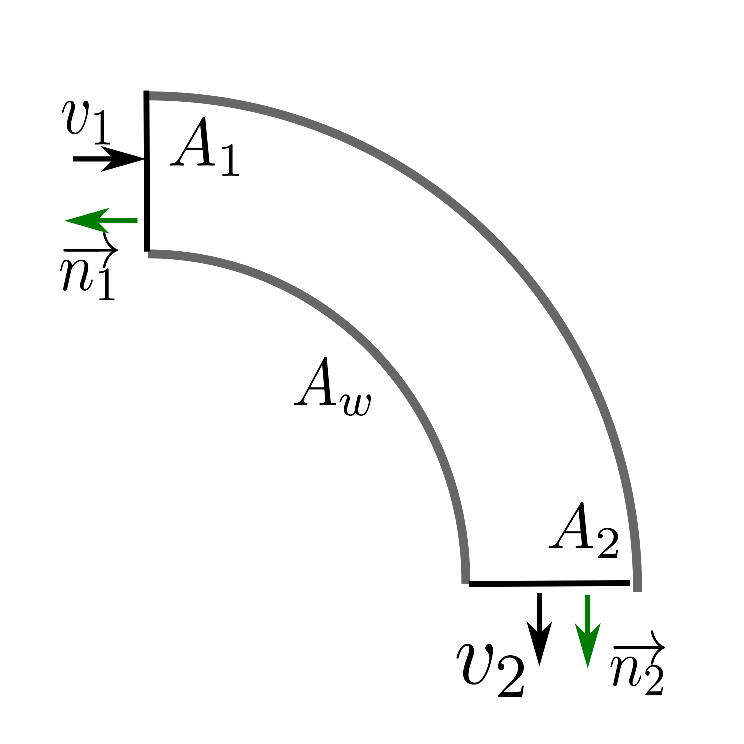
\includegraphics[width=5cm]{horizontal_tube.eps}
\caption{水平弯管}\label{fig:511}
\end{figure}

如上图所示,已知管的入口横截面和出口横截面面积分别为$A_1$,$A_2$。
进水口速度为$v_1$,压强为$p_1$,流体假设为理想不可压定常流,密度为$\rho$,求流体对水平弯管的作用力。

解:坐标系选为地面系,控制体选为水平弯管,由连续性方程有:
\begin{equation}\label{eq:51H1}
v_1A_1=v_2A_2
\end{equation}
由Bernoulli方程有:
\begin{equation}\label{eq:51H2}
\frac{1}{2}v_1^2+\frac{p_1}{\rho}=\frac{1}{2}v_2^2+\frac{p_2}{\rho}
\end{equation}
由动量守恒积分方程
\begin{equation*}
\oiint\limits_{\Sigma} \v{T_n} dA+\iiint\limits_{\tau}\rho\v{f}\d\tau
-\oiint\limits_{\Sigma}\rho\v{v}(\v{v}\cdot\v{n})dA=0
\end{equation*}
上式中$T_n$是表面力,在$A_i$面上($i=1,2$),由于$T_n=-p_i\v{n_i}$,而在$A_w$面上,设所求的作用力为$\v{F}$则弯管对流体的
作用力为$-\v{F}$,因此第一项化简为$-\v{F}-p_1A_1\v{n_1}-p_2A_2\v{n_2}$。
上式第二项为体积力的贡献,即为重力势$\rho \v{g} \tau$,其中$\tau$为管内流体体积。
上式第三项为动量的输运项,考虑到$\v{v_1}=-v_1\v{n_1},\v{v_2}=v_2\v{n_2}$,可得到第三项(不带前面负号)为
$\rho v_1^2 A_1\v{n_1}+\rho v_2^2 A_2\v{n_2}$,因此动量守恒方程最终化为
\begin{equation}\label{eq:51H3}
\v{F}=\rho g \tau -p_1A_1\v{n_1}-p_2A_2\v{n_2} - \rho v_1^2 A_1\v{n_1} - \rho v_2^2 A_2\v{n_2}
\end{equation}
从式\eqref{eq:51H1}和式\eqref{eq:51H2}中解出$v_2,p_2$代入式\eqref{eq:51H3}中得到流体对水平弯管的作用力为:
\begin{equation}
\v{F}=\rho \v{g} \tau -p_1A_1\v{n_1}-(\frac{\rho v_1^2}{2}-\frac{\rho v_1^2A_1^2}{2A_2^2}+p_1)A_2\v{n_2} - \rho v_1^2 A_1\v{n_1} - \rho \frac{v_1^2A_1^2}{A_2^2} A_2\v{n_2}
\end{equation}
若$A_1=A_2$,则可推出$v_1=v_2,p_1=p_2$,作用力化简为:
\begin{equation}
\v{F}=\rho \v{g} \tau -(p_1+\rho v_1^2)(\v{n_1}+\v{n_2})
\end{equation}
由于$\v{g}$与水平弯管平面垂直,当$\v{n_1}=-\v{n_2}$,即管是直的,作用力达到最小,这对消防员灭火时使用喷水管的方法具有一定指导意义。

2.叶轮机械的功率
\begin{figure}[!ht]
\centering
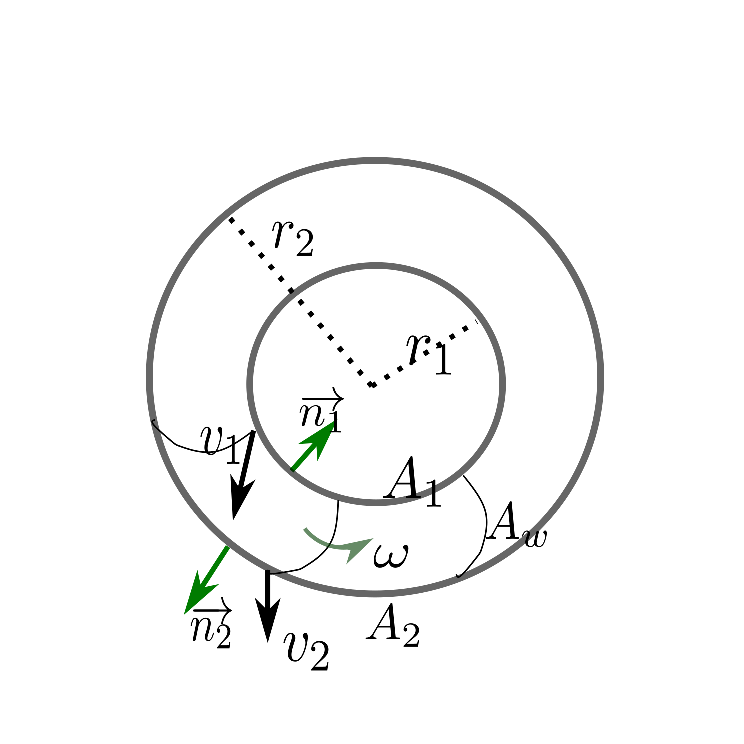
\includegraphics[width=5cm]{turbine_power.eps}
\caption{叶轮机械示意图}\label{fig:512}
\end{figure}

叶轮机械的简化模型如上图所示,转动角速度为常数$\v{\omega}$,纵向$\v{e_z}$设为单位长度,
流体假设为理想不可压定常流,且速度分布均匀,我们取旋转中的叶轮机为参考系,
以叶轮机为控制体。由于我们选的参考系是非惯性系,需要考虑惯性力项,为此首选考虑速度的分解,设$\v{u}$是叶轮机上某位置对地速度,
$\v{w}$是该位置流体微团相对叶轮机的速度,$\v{v}$是该位置流体微团对地速度,速度分解关系如下图所示:
\begin{figure}[!ht]
\centering
%LaTeX with PSTricks extensions
%%Creator: inkscape 0.92.2
%%Please note this file requires PSTricks extensions
%\documentclass{article}
%\pagestyle{empty}
%\usepackage{tikz}
%\begin{document}
 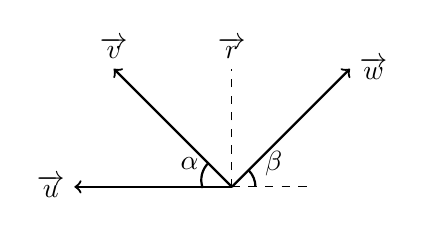
\begin{tikzpicture}
  \draw[thick,->] (2,0) -- (0,0);
  \draw[thick,->] (2,0) -- (3.5,1.5);
  \draw[thick,->] (2,0) -- (0.5,1.5);
  \draw[thick] (23mm,0mm) arc [start angle=0, end angle=45, radius=3mm]; %beta
  \draw[thick] (17mm,3mm) arc [start angle=135, end angle=200, radius=3mm]; %alpha
  \draw (0,0) node[anchor=east] {$\overrightarrow{u}$};
  \draw (3.5,1.5) node[anchor=west] {$\overrightarrow{w}$};
  \draw (0.5,1.5) node[anchor=south] {$\overrightarrow{v}$};
  \draw (1.7,0.3) node[anchor=east] {$\alpha$};
  \draw (2.3,0.3) node[anchor=west] {$\beta$};
  \draw[dashed] (2,0) -- (3,0);
  \draw[dashed] (2,0) -- (2,1.5);
  \draw (2,1.5) node[anchor=south] {$\overrightarrow{r}$};  
  \end{tikzpicture}
%\end{document}
\caption{速度分解关系示意图}\label{fig:513}
\end{figure}
且满足$\v{v}=\v{w}+\v{u}$,其中$\beta$被称为安装角,$\alpha$为进气(出气)角。该位置流体微团对地的加速度
\begin{equation}
\v{a}=\v{\omega}\times(\v{\omega}\times \v{r})+2\v{\omega}\times \v{w}
\end{equation}
化简可得:
\begin{equation}\label{eq:51acc}
-\v{a}=\omega^2 \v{r} +2\v{w}\times \v{\omega}
\end{equation}
由动量矩守恒积分方程有:

\begin{equation}\label{eq:momentumConservation}
\underbrace{\iiint\limits_D \rho(\v{r}\times (\v{f}-\v{a}))d\tau}_{I_1}+
\underbrace{\oiint\limits_{\Sigma} (\v{r}\times\v{T_n})dA}_{I_2}-
\underbrace{\oiint\limits_{\Sigma} (\v{r}\times \rho\v{w})(\v{w}\cdot\v{n})dA}_{I_3}=0
\end{equation}

\begin{align}
I_1= & \iiint\limits_D \rho(\v{r}\times (-\v{a}))d\tau, \v{f}=\v{g}\text{与叶轮机平面垂直} \nonumber\\
= & \iiint\limits_D \rho(\v{r}\times (\omega^2 \v{r} +2\v{w}\times \v{\omega}))d\tau,\text{代入}\eqref{eq:51acc}\nonumber\\
= & 2\iiint\limits_D \rho((\v{r}\cdot\v{\omega})\v{w}-(\v{r}\cdot\v{w})\v{\omega})d\tau, A\times (B\times C)=(A\cdot C)B-(A\cdot B)C\nonumber\\
= & -2\iiint\limits_D \rho (\v{r}\cdot\v{w})\v{\omega}d\tau\nonumber\\
= & -2\left(\int_{r_1}^{r_2} rdr\right)\left(\int_0^{2\pi}\rho(\v{r}\cdot\v{w})d\theta\right)\v{\omega}, \text{按柱坐标积分}\nonumber\\
= & -Q_m(\omega r_2^2-\omega r_1^2)\v{e_z}, \text{质量流量的定义}Q_m=\int_0^{2\pi}\rho(\v{r}\cdot\v{w})d\theta\nonumber\\
= & -Q_m(u_2r_2-u_1r_1)\v{e_z},\text{入口和出口处牵连速度为圆周运动线速度} \label{eq:51I1}\\
\end{align}

由于相对速度$\v{u}$沿侧面切线方向,与$\v{n}$点积为零,侧面积分为零,$I_3$中面积分只需考虑$A_1\cup A_2$,
由连续性方程:$Q_m=-\rho_1 \v{w_1}\cdot \v{n_1} A_1=\rho_2 \v{w_2}\cdot \v{n_2} A_2$。
同样由图\ref{fig:513}的几何关系,在$A_1$面上有
$\v{r}\times \v{w}=-r_1 w_1 \cos\beta_1 \v{e_z}$,
因此对$A_1$上的面积分我们有
\begin{equation}
\oiint\limits_{A_1} (\v{r}\times \rho\v{w})(\v{w}\cdot\v{n})dA=Q_m r_1 w_1 \cos\beta_1 \v{e_z}
\end{equation}
同理可求出$A_2$上的面积分为$-Q_m r_2 w_2 \cos\beta_2 \v{e_z}$,进而得到
\begin{equation}\label{eq:51I3}
I_3=Q_m (r_1 w_1 \cos\beta_1 - r_2 w_2 \cos\beta_2) \v{e_z}
\end{equation}

$I_2$包含叶片侧面对流体的力矩,通过式\eqref{eq:momentumConservation}可以求出该力矩。
由于是理想流体,$\v{T_n}=-p\v{n}$与$\v{r}$平行,因此进出口面$A_1,A_2$无力矩,于是我们得到:
\begin{align*}
\v{M}=& I_2 \\
=& -I_1+ I_3 \\
=& Q_m (u_2r_2-u_1r_1)\v{e_z} + Q_m (r_1 w_1 \cos\beta_1 - r_2 w_2 \cos\beta_2) \v{e_z}, \text{式\eqref{eq:51I1}和\eqref{eq:51I3}} \\
=& Q_m[r_2(u_2-w_2\cos\beta_2)-r_1(u_1-w_1\cos\beta_1)]\v{e_z}\\
=& Q_m(r_2v_2\cos\alpha_2 - r_1 v_1\cos\alpha_1)\v{e_z},\text{图\ref{fig:513}中几何关系} \\
\end{align*}
进一步我们可求出叶轮机的功率$N=\v{M}\cdot\v{\omega}$。

\begin{thebibliography}{9}
\bibitem{mixedProduct} \href{https://en.wikipedia.org/wiki/Triple_product}{https://en.wikipedia.org/wiki/Triple\_product}
\bibitem{velocityGradient}\href{http://www.continuummechanics.org/velocitygradient.html}{http://www.continuummechanics.org/velocitygradient.html}
\bibitem{angularVelocityTensor}\href{https://en.wikipedia.org/wiki/Angular_velocity#Angular_velocity_tensor}{https://en.wikipedia.org/wiki/Angular\_velocity\#Angular\_velocity\_tensor}
\bibitem{CylindricalCoordinates}\href{https://en.wikipedia.org/wiki/Divergence#Cylindrical_coordinates}{https://en.wikipedia.org/wiki/Divergence\#Cylindrical\_coordinates}
\bibitem{CurlFormular}\href{https://en.wikipedia.org/wiki/Curl_(mathematics)}{https://en.wikipedia.org/wiki/Curl\_(mathematics)}
\bibitem{FundamentalSolution}\href{https://en.wikipedia.org/wiki/Fundamental_solution}{https://en.wikipedia.org/wiki/Fundamental\_solution}
\bibitem{GreenFunction}\href{https://en.wikipedia.org/wiki/Green\%27s_function#Green.27s_functions_for_the_Laplacian}{https://en.wikipedia.org/wiki/Green\%27s\_function\#Green.27s\_functions\_for\_the\_Laplacian}
\end{thebibliography}
\end{document}